
\section{Simultaneous Localization and Mapping (SLAM)}
\subsection{Motivations and general description}
SLAM is the computation problem of constructing and updating a map of an unknown environment whole simultaneously keeping track of an agent's location within it, using measurements $z_{1:t}$ and the controls $u_{1:t}$ up to time $t$. This data is gathered by the robot's propioceptive and exteroceptive sensors. SLAM is difficult because both the estimated path and extracted features are corrupted by noise. We assume that the initial location of the robot is known and the others are not.\\ \\
According to this terminology, the full SLAM problem consists of estimating the joint posterior probability of the robot path $x_{1:t}$ and the map $m$, from the odometry $u_{1:t}$ and observations $z_{1:t}$
$$p(x_{1:t}, m|z_{1:t}, u_{1:t})$$
The online SLAM problem aims to estimate the joint posterior over the robot's current pose $x_t$ and the map $m$, from the data $z_{1:t}, u_{1:t}$
$$p(x_t, m|z_{1:t}, u_{1:t})$$
This is represented graphically in Figure 13.4.

\subsection{Extended Kalman Filter localization with map uncertainty: EKF SLAM}
EKF SLAM shares some similarities with EFK localization. First, we assume the existence of a feature-based map
$$m = \{m_1,...,m_N\}$$
where $m_i$ is the $i$-th landmark. We denote the global frame coordinates of the $i$-th point landmark $m_i$ with $(m_{i,x}, m_{i,y})$. Moreover, we assume the availability of a sensor that can measure the range and bearing pair $z = (r, \phi)$ of a landmark relative to the robot's local coordinate frame. Furthermore, in order to keep track of the uncertainty over the robot's pose $x_t$ and the map $m$, we use Markov probabilistic models for motion, $p(x_t|x_{t-1}, u_{t-1})$, and perception, $p(z_t|x_t,m)$. These models, as well as our initial beliefs over the robot's pose and the map are assumed to be Gaussian.

\textbf{Similarly to EKF localization}, EKF SLAM aims to estimate the robot pose $x_t = (x, y, \theta)$ at time $t$ with the following procedure:

\begin{itemize}
    \item A set $z_t = \{z_t^1, z_t^2,...,\}$ of range and bearing pairs $z_t^i = (r_t^i, \phi_t^i)$ is measured by the robot through its sensor.
    \item A landmark $m_j$ is associated with each measurement $z_t^i$. We define the correspondence variable $c_t^i \in \{1,...,N+1\}$, such that $c_t^i = j$ if the $i$-th measurement $z_t^i$ corresponds to the $j$-th landmark, and $c_t^i = N+1$ if no landmark corresponds to the $i$-th measurement.
    \item Given those new measurements and associations, the resulting posterior distribution on the robot's pose is computed.
\end{itemize}

We distinguish between two versions of EKF SLAM:
\begin{itemize}
    \item The correspondence variables $c_t^i$ are known, i.e.: given a measurement, we know the corresponding landmark (idealistic case).
    \item The correspondence variables $c_t^i$ and the number of landmarks $N$ are unknown. The algorithm must account for this uncertainty (usual case).
\end{itemize}

\textbf{Unlike EKF localization}, EKF SLAM does not assume knowledge of the landmarks' coordinates $\{(m_{i,x}, m_{i,y})\}_{i=1}^N$. Hence, EKF SLAM estimates the coordinates of all landmarks.

\subsection{EKF SLAM with known correspondences}
In the case of known correspondences, the approach to track the uncertainty over both the robot's pose $x_t$ and the map $m$ is to consider an augmented state $y_t \in \mathbb{R}^{3+2N}$ defined as:

\begin{equation}
    y_t := 
    \begin{pmatrix}
    x_t \\
    m
    \end{pmatrix}
    = (x, y, \theta, m_{1,x},m_{1,y},...,m_{N,x},m_{N,y})^T
\end{equation}

Hence, the augmented state $y_t$ comprises the robot's pose $x_t$ and the representation of the map $m$ through its landmarks' coordinates in the global coordinate frame. At time $t$, given all the measurements $z_{1:t}$ and all the inputs $u_{1:t}$ up to time $t$, the goal is to calculate the online posterior distribution over the augmented state $y_t$:
$$p(y_t|z_{1:t}, u_{1:t})$$

Note that here we do not compute a posterior over the variables $c_t$, since we assume known correspondences.

To apply the EKF machinery, we treat SLAM as an estimation problem and assume all landmarks are static. In order to cast everything into an EKF filtering problem, we need to specify motion and sensing models. Assume linear motion model with state $x_t = (x, y, \theta)$:

\begin{equation}
    y_t = g(u_t, y_{t-1}) + \epsilon_t, \> \>
    \epsilon_t \sim N(0,R_t), \> \>
    G_t := J_g(u_t, y_{t-1})
\end{equation}

where $g(u_t,y_{t-1})$ is the dynamics of our entire state space, including the pose of the robot and the position of the landmarks. Hence, $g$ is a 3 + 2$N$ vector  whose first three components describe the dynamics of the robot and the rest 2$N$ are all zeros since the landmarks are static. The covariances between the 3 + 2$N$
variables on system dynamics are stored in the covariance matrix, $R_{t}$. For the noise model of our dynamics, Rt has dimension 3 + 2$N$ by 3 + 2$N$, and, for similar reason, only the upper left 3 by 3 sub-matrix representing the noise in robot pose is nonzero. The matrix $G_{t}$ is the Jacobian of $g$ at $(u_{t}, y_{t-1})$.

We instantiate the measurement model in the same way as for EKF localization and assume a range and bearing measurement model:

\begin{equation}
    \hat{z}_{t}^{i} = 
        \begin{pmatrix}
            \sqrt{(m_{j,x} - x)^{2} 
            + (m_{j,x} - x)^{2}} \\
            atan2(m_{j,y} - y, 
            m_{j,x} -x) - \theta
            \end{pmatrix} 
            + \delta_{t} := h(y_{t},j) + \delta_{t}
\end{equation}
where \\
\begin{equation*}
    \delta_{t} \sim N(0,Q_{t}),\  Q_{t} = 
    \begin{pmatrix}
    \sigma^{2}, 0 \\
    0, \sigma_{\phi}^{2}
    \end{pmatrix}
    \ \text{and} \ c^{i}_{t} = j
\end{equation*}
The function that maps the states into the measurement $z^{i}_t$ is given by range and bearing, so this is identical to the case of EKF localization. The only difference is that we are mapping a much larger state vector with some noise into a 2D vector. As it was the case for the motion model, we approximate the measurement model according to a linear function by taking a Taylor expansion around the mean of the predicted belief over $y_{t}$.
\begin{equation}
    h(y_{t},j) \approx h(\bar{\mu}_{t}, y) + H^{i}_{t}(y_{t} - \bar{\mu}_{t})
\end{equation}
where
\begin{equation*}
    H^{i}_{t} := \frac{\partial{h(\bar{\mu}_{t}, j)}}{\partial{y_{t}}}
\end{equation*}

When taking the derivative of the function $h$ to obtain the Jacobian, we will have zero terms because we are taking derivatives with respect to state variables that do not impact the measurement model. Then, the derivative of $h$ with respect to $x_{t}$ and $m_{j}$ can be expressed as
\begin{equation}
    h^{i}_{t} = \frac{\partial{h(\bar{\mu}_{t},j)}}{\partial{(x_{t},m_{j})}} = 
    \begin{pmatrix}
    \frac{\bar{\mu}_{t,x} - \bar{\mu}_{j,x}}{\sqrt{q_{t,j}}},\
    \frac{\bar{\mu}_{t,y} - \bar{\mu}_{j,y}}{\sqrt{q_{t,j}}},\
    0,\
    \frac{\bar{\mu}_{j,x} - \bar{\mu}__{t,x}}{\sqrt{q_{t,j}}},
    \frac{\bar{\mu}_{j,y} - \bar{\mu}_{t,y}}{\sqrt{q_{t,j}}} \\
    \frac{\bar{\mu}_{j,y} - \bar{\mu}_{t,y}}{q_{t,j}}, \
    \frac{\bar{\mu}_{j,x} - \bar{\mu}_{t,x}}{q_{t,j}}, \
    -1,\ 
    \frac{\bar{\mu}_{t,y} - \bar{\mu}_{j,y}}{q_{t,j}}, \
    \frac{\bar{\mu}_{t,x} - \bar{\mu}_{j,x}}{q_{t,j}} \
    \end{pmatrix}
\end{equation}
where $\bar{\mu}_{t,x}$ and $\bar{\mu}_{t,y}$ are the current estimations of the x and y coordinates of the robots, and $\bar{\mu}_{j,x}$ and $\bar{\mu}_{j,y}$. are the expected values of x and y coordinates with respect to the $j^{\text{th}}$ landmark. And
\begin{equation*}
    q^{t}_{j} \ := (\bar{\mu}_{j,x} - \bar{\mu}_{t,x})^{2} + (\bar{\mu}_{j,y} - \bar{\mu}_{t,y})^{2}.
\end{equation*}


\setcounter{MaxMatrixCols}{20}
Define $F \in \mathbb{R}^{5 \times (3 +2N)}$ as
\begin{equation}
    F^{i}_{j} = 
    \begin{pmatrix}
    1 & 0 & 0 & \ 0 \cdots 0 \ & 0 & 0 \ & 0 \cdots 0 \\
    0 & 1 & 0 & \ 0 \cdots 0 \ & 0 & 0 \ & 0 \cdots 0 \\
    0 & 0 & 1 & \ 0  \cdots 0 \ & 0 & 0 \ & 0 \cdots 0 \\
    0 & 0 & 0 & \ 0  \cdots 0 \ & 1 & 0 \ & 0 \cdots 0 \\
    0 & 0 & 0 & \ \underbrace{0  \cdots 0}_{2j-2} \ & 0 & 1 \ & \underbrace{0 \cdots 0}_{2N-2j} \\
    \end{pmatrix}
\end{equation}


Then, we have the following factorization: 
\begin{equation}
    H^{i}_{t} = h^{i}_{t} F_{x,j}
\end{equation}
The following step is initializing the algorithm. Usually the initial pose is taken to be the origin of the
coordinate system. In this case, the map is unknown. The initial belief is then expressed as
\begin{equation}
\mu_{0} = (0, \ 0, \ \dots \ , \ 0)^{T}    
\end{equation}
Although an arbitrary choice, taking the initial belief as a zero vector can greatly reduce computation in later operations. The next step is initializing the covariance matrix for augmented state vectors. Assuming that the robot has known pose and is at the origin of an unknown map, we have zero covariances for the top left 3*3
block of the matrix as initialization for pose variables. Since the locations of landmarks are unknown, the covariances of landmarks with respect to themselves are taken to be infinite, which is represented by large numbers in practice. In addition, there is no information on the cross correlations between different landmarks, and hence the off-diagonal elements in the covariance matrix are initialized as zeros.
\begin{equation}
    \Sigma_{0} = \begin{pmatrix}
    0 & 0 & 0 & 0 & \cdots & 0 \\
    0 & 0 & 0 & 0 & \cdots & 0 \\
    0 & 0 & 0 & 0 & \cdots & 0 \\
    0 & 0 & 0 & \infty & \cdots & 0 \\
    \vdots & \vdots & \vdots & \vdots & \ddots & \vdots \\
    0 & 0 & 0 & 0 & \cdots & \infty \\
    \end{pmatrix}
\end{equation}
When the robot observes a landmark for the first time, it initializes the position for that landmark based units estimated current position obtained using range and bearing measurement model. Hence the landmark estimates $(\bar{\mu}_{j,x},\bar{\mu}_{j,y})^{T}$ can be determined as:
\begin{equation}
    \begin{pmatrix}
    \bar{\mu}_{j,x} \\
    \bar{\mu}_{j,y}
    \end{pmatrix}
    = \begin{pmatrix}
    \bar{\mu}_{t,x}\\
    \bar{\mu}_{j,y}
    \end{pmatrix}
    +
    \begin{pmatrix}
    r^{i}_{t}\text{cos}(\phi^{i}_{t} + \bar{\mu}_{t,\theta}) \\
    r^{i}_{t}\text{sin}(\phi^{i}_{t} + \bar{\mu}_{t,\theta})
    \end{pmatrix}
\end{equation}
The first term on the right-hand side is the estimated position of the robot. In the second term, $r^{i}_{t}$, represents the distance between robot and landmark, and the trigonometry terms on the relative angles stores the directional information. EKF SLAM algorithm, shown in Figure (13.5), is very similar to the EKF localization algorithm. The biggest difference is that new landmarks may be discovered and needs to be accounted for. Other main differences are augmented state vector, augmented dynamics (with trivial dynamics for the landmarks), and augmented measurement Jacobian. Also similar to EKF localization, this algorithm contains a Bayesian filter and the prediction step propagates the expected value of our state factor, which is an augmented state vector, and the covariance of our predicted belief using the motion model. Since landmarks are assumed to be static, only the first three elements of the state vector and the top left 3 by 3 block of the covariance matrix are updated. Therefore, only the mean of the covariance belief is manipulated in the prediction step in accordance to the motion model. And the step only affects elements with beliefs
distribution related to a robot pose. Afterwards, information about the measurements will be incorporated. Each measurement is processed
sequentially as in EKF localization. With the assumption of known correspondence variables, once measurements $z^{t}_{t}$ are obtained, we have correspondence variable that shows $c^{i}_{t}$ measurement corresponding to the landmark $j$. If the landmark $j$ has not been seen before, its position will be initialized. The rest of steps
are the same as in EKF localization. Time and memory complexity for EKF SLAM algorithm are $O(N^{2})$.

\subsection{EKF SLAM with unknown correspondences}
The general idea of EKF SLAM with unknown correspondences is to use maximum likelihood estimation to decide the measurement correspondences during the measurement step. The rest of the algorithm follows similar to the EKF SLAM algorithm assuming known correspondences discussed previously.

%% Including graphics
\begin{center}
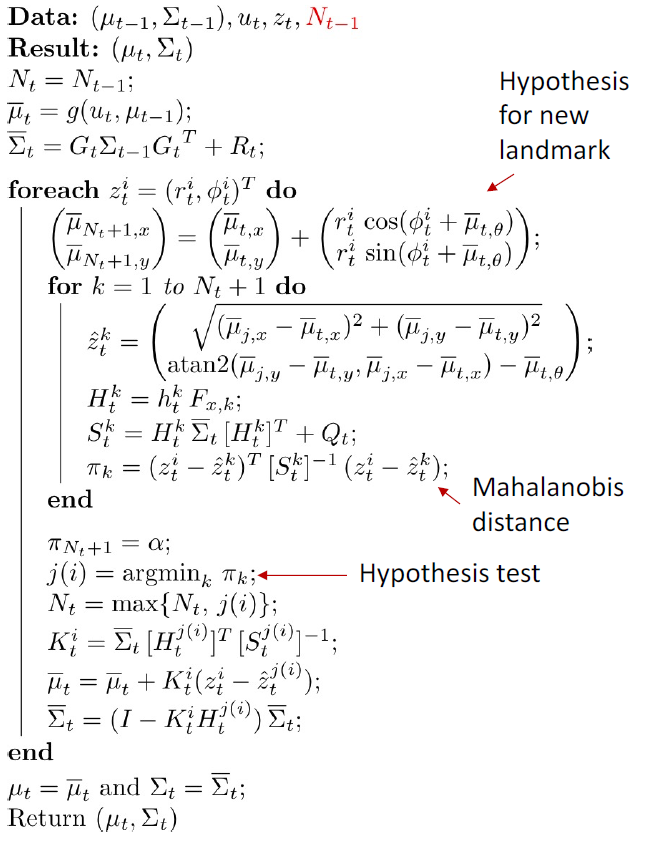
\includegraphics[scale = 0.6]{ekf_slam.png}\\
Figure 13.5: Pseudocode for EKF SLAM with unknown correspondences.
\end{center}


This algorithm’s more general applicability comes at the cost of being less robust.
The key difference in the interface of the algorithm is that, in addition to estimating the positions of each of the landmarks, it also may estimate the number of landmarks. Therefore we consider $N_t$, the estimated number of landmarks at time t to be an input. At the measurement step, we loop over all measurements $z_{t}^i$. Then, for each of the $N_t$ landmarks, we calculate the likelihood of each $z_t^i$, corresponding to each landmark.


The first step is to form $\hat{z}_{t}^{k}$, the expected measurement at time $t$ given our belief of landmark $k, \bar{\mu},  k$. In the case where we receive range and bearing measurements, this is:

\begin{equation}
    \hat{z}_{t}^{k} = 
        \begin{pmatrix}
            \sqrt{(\bar{\mu}_{k,x} - \bar{\mu}_{t,x})^{2} 
            + (\bar{\mu}_{k,y} - \bar{\mu}_{t,y})^{2}} \\
            atan2(\bar{\mu}_{k,y} - \bar{\mu}_{t,y}, 
            \bar{\mu}_{k,x} - \bar{\mu}_{t,x}) - \bar{\mu}_{t,\theta}
        \end{pmatrix}
\end{equation}

We can then calculate the likelihood $z_{t}^i$ corresponding to our landmark by taking the Mahalanobis distance between $z_{t}^i$ and $z_{t}^k$. The Mahalanobis distance corresponds to the z-score of the measurement $z_{t}^i$ under
our measurement model centered at $z_{t}^k$. Using the notation similar to before, we form

\begin{equation}
    H_t^k = h_t^k F_{x,k}
\end{equation}

which is the Jacobian of the measurement model with respect to the kth landmark at time $t$. We then use this Jacobian to project the error covariance of the state at time $t$ to the error covariance of our measurement:

\begin{equation}
    S_t^k = H_t^k \bar{\Sigma}_{t} \big[ H_t^k\big]^T + Q_t  
\end{equation}

Finally, we calculate the Mahalanobis distance as:
\begin{equation}
    \pi_k = (z_t^i - \hat{z}_t^k) [S_t^k]^{-1} (z_t^i - \hat{z}_t^k)
\end{equation}

We can then estimate $j(i)$, the correspondence of measurement $Z_t^i$ as:

\begin{equation}
    j(i) = \argmin_{k \in {1, \dots, N_t + 1}} \pi_k
\end{equation}

We also set a threshold distance $\pi_{N_t + 1} = \alpha$. If it happens that $\alpha$ is the minimum distance between measurement $z_t^i$ and each landmark, then we treat $z_t^i$ as having come from a new landmark, $N_{t} + 1$, and we initialize its belief as the expected position given the measurement $z_t^i$:

\begin{equation}
    \begin{pmatrix}
        \bar{\mu}_{N_t + 1, x} \\
        \bar{\mu}_{N_t + 1, y}
    \end{pmatrix} = 
    \begin{pmatrix}
        \bar{\mu}_{t, x} \\
        \bar{\mu}_{t, y}
    \end{pmatrix} +
    \begin{pmatrix}
        r_t^i \cos(\phi_t^i + \bar{\mu}_{t,\theta}) \\
        r_t^i \sin(\phi_t^i + \bar{\mu}_{t,\theta}) 
    \end{pmatrix}
\end{equation}

We would also increment $N_t$ by 1. After we have formed the correspondence function $j(i)$, we can simply proceed with the measurement step as before, to update our beliefs. The full pseudo-code for the algorithm is shown in Figure 13.5.

As mentioned before, this algorithm’s broader applicability comes at the cost of being less robust. In particular, extraneous measurements can result in the creation of fake landmarks, which will then propagate forward to future steps uncorrected. Furthermore, the EKF can diverge if non-linearities are large.

There are several techniques to mitigate these issues, such as:

\begin{itemize}
    \item  Outlier rejection schemes [3] employing provisional landmark lists, etc.
    \item Strategies to enhance the distinctiveness of landmarks which may involve prior knowledge or assumptions, such as spatial arrangements, signatures, geometric constraints, etc.
\end{itemize}

However, the central dilemma of EKF SLAM is that accurate localization typically requires dense maps, while EKF requires sparse maps due to the quadratic complexity of updates.

%% ---
% ADD NOTES HERE



%% ---